
\chapter{A Combinatorial Miscellany}


%\section{Domino Tilings}


%\section{Permutations}

\section{Perfect Matchings and Pfaffian Orientations}
Refer to \href{https://youtu.be/ydCWu6aiAxE?si=v91XmPDjM3qkfGKw}{https://youtu.be/ydCWu6aiAxE?si=v91XmPDjM3qkfGKw}. 
\section{Graphs and Trees}
We start with a standard result on graphs.
\begin{theorem}
    Let $G$ be a simple, connected graph on $n$ vertices. Then the following are equivalent.
    \begin{enumerate}
        \item $G$ is minimally connected.
        \item $G$ has $n-1$ edges.
        \item $G$ has no cycles.
    \end{enumerate}
    \label{t:G&T_Main}
\end{theorem}
\begin{proof}
If $G$ is minimally connected, then removing any edge of $G$ would disconnect it. This means that each edge of $G$ is a bridge. Since G is connected, it must have at least $n-1$ edges. If G had more than $n-1$ edges, then removing any additional edge would not disconnect $G$, contradicting the minimality assumption. Therefore, $G$ must have exactly $n-1$ edges. This proves that $(1)\implies (2)$. If G has $n-1$ edges and $n$ vertices, then it is a tree. Trees are acyclic by definition, so $G$ has no cycles. This proves $(2)\implies (3)$. Finally, if G has no cycles, then it is a tree. Trees are minimally connected, meaning that removing any edge disconnects the graph. Therefore, $G$ is minimally connected. This proves $(3)\implies (1)$. Having formed a loop of implications, we are done.
\end{proof}
Recall the following definitions. Graphs satisfying any one of the properties in \cref{t:G&T_Main} are called trees. Additionally, graphs whose connected components are trees are called forests. More importantly, a tree on $n$ vertices is called a labeled tree if each vertex gets a label from the set $[n]$. 
\par
With this background at hand, we are interested in counting $T_n$, the number of labeled trees on $n$ vertices. From the figure below it is clear that $T_1,T_2,T_3$ and $T_4$ are $1,1,3$ and $16$. One might guess that $T_n=n^{n-2}$. In fact this is precisely what we want to prove.
\begin{figure}[H]
    \centering
    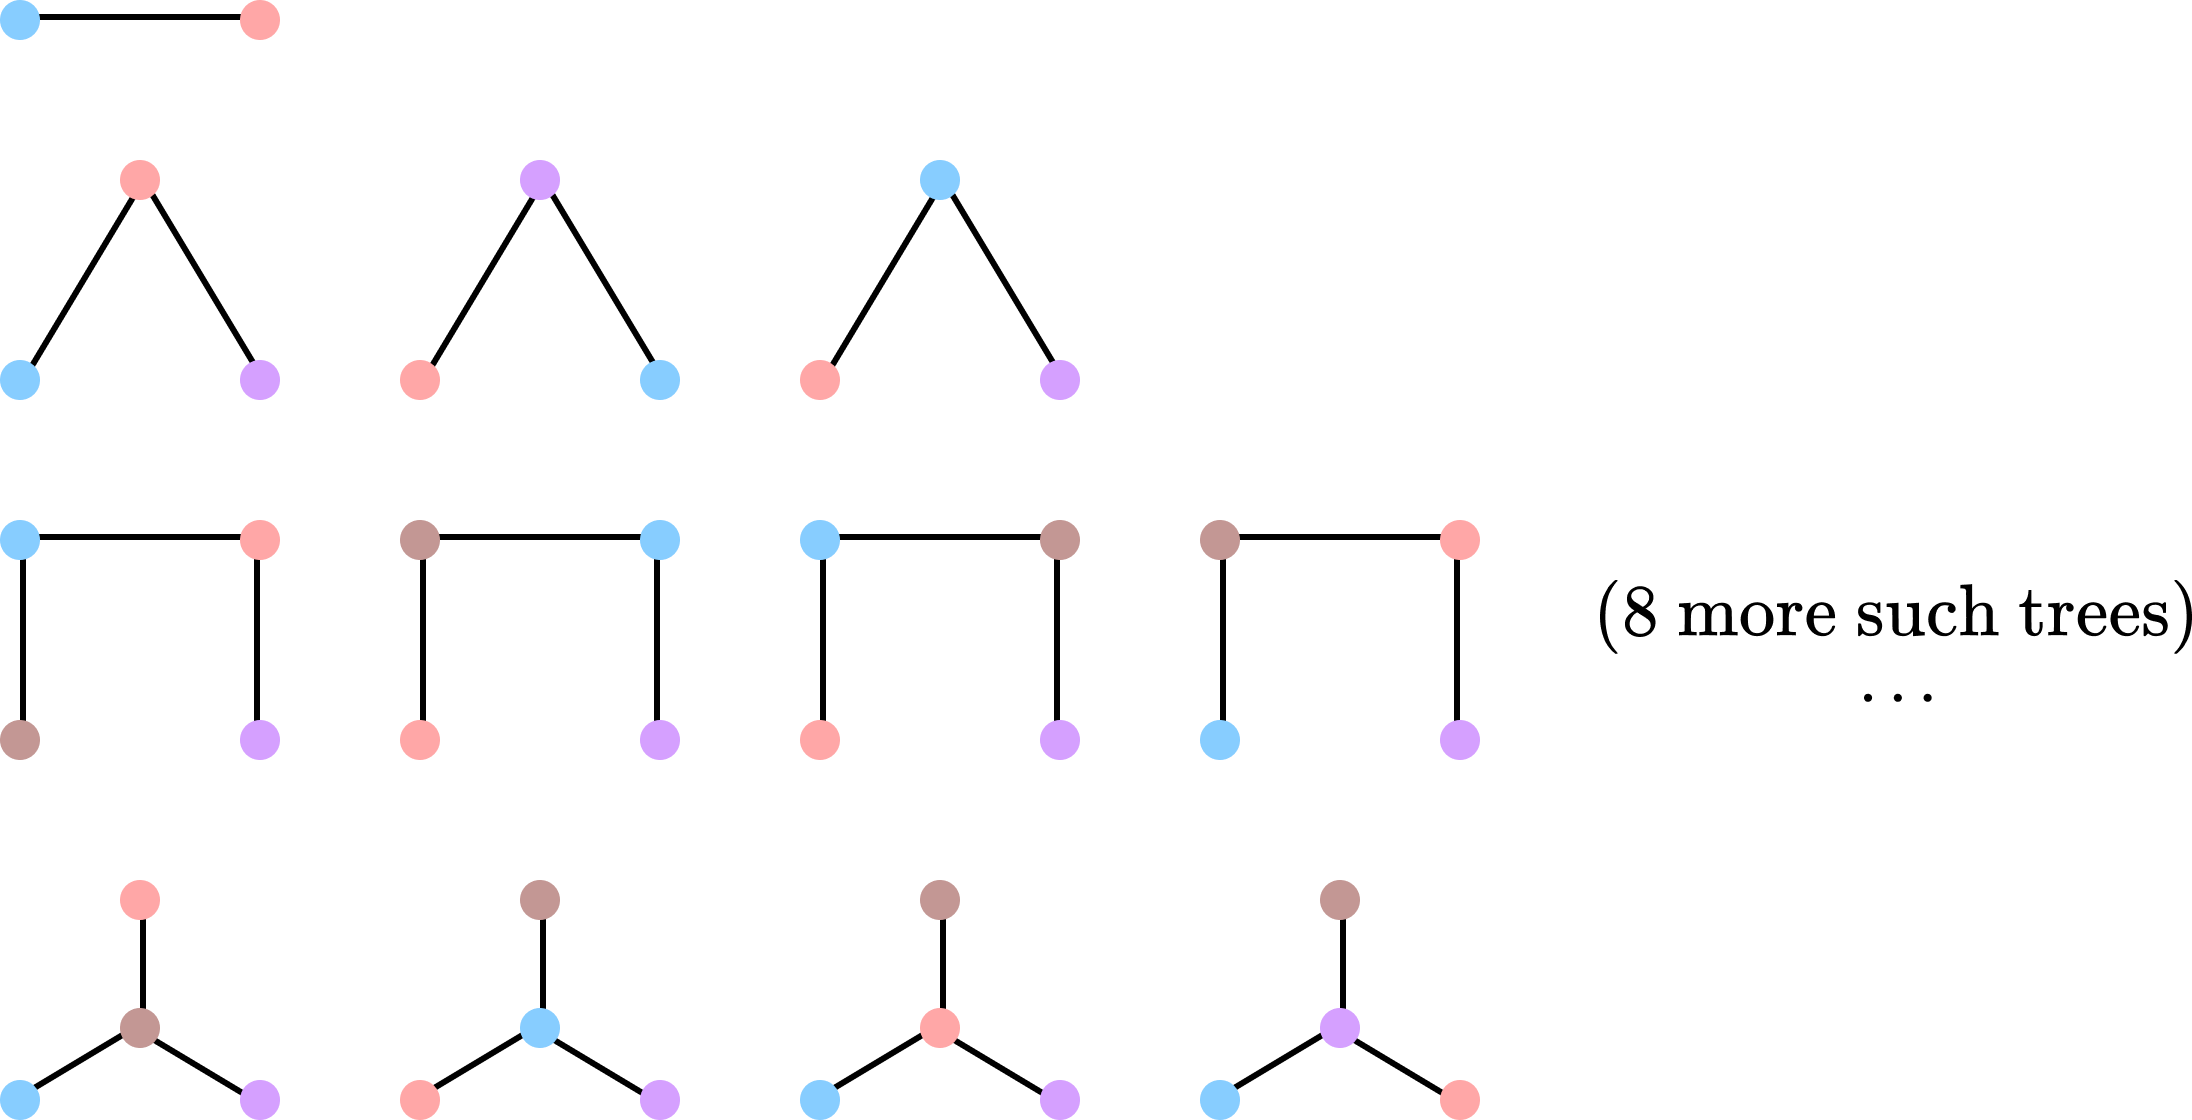
\includegraphics[width=0.9\linewidth]{Images/Figure29.png}
    \caption{}
    \label{f:Cayley Trees}
\end{figure}

\begin{theorem}[Cayley's Formula]
If $T_n$ denotes the number of labeled trees on $n$ vertices, then
    \[
    T_n = n^{n-2}.
    \]
    \label{t:Cayley's Formula}
\end{theorem}
\begin{proof}
\end{proof}
\begin{theorem}
The number of rooted forests on $[n]$ is $(n+1)^{n-1}$.
\end{theorem}
\begin{proof}
\begin{comment}
Let $F(n)$ be the set of all rooted forests on $[n]$. Let $T(n)$ be the set of all labeled trees on $[n]$. We claim that \[
|F(n)|=|T(n+1)|=(n+1)^{n-1} \quad \text{(the second equality follows from } \cref{t:Cayley's Formula}\text{)}
\]
\end{comment}
\end{proof}
We conclude this section with a result whose proof we shall omit but see \cref{t:Cayley's Formula} as a consequence of. 
\begin{theorem}
    The number of rooted forests on $[n]$ with $k$ components is \[
    \binom{n-1}{k-1}n^{n-k}.
    \]
\end{theorem}
Notice how setting $k\to 1$ and multiplying the result by $n$ (to account for the $n$ choices of roots) gives \cref{t:Cayley's Formula} back. 
\section{Permutations Revisited}

%\section{Symmetric Functions}







\endinput
